\section{Experimentos}


%*******************************************************************
\begin{frame}{Experimento 1: Verificação autoral}
\fontsize{3.0mm}{4.0mm}\selectfont
\begin{block}{Publicação 1}
	CUSTÓDIO, J. E.; PARABONI, I. Similaridade de Textos aplicada à Verificação Autoral.
	In: 1st International Congress on Digital Humanities in Rio de Janeiro. [S.l.]: Fundação
	Getúlio Vargas, 2018.
\end{block}

\begin{block}{Verificação autoral ou atribuição por similaridade}
	\begin{itemize}
		\item Deseja-se saber se pares de documentos foram escritos pelo mesmo autor. \cite{Koppel2012}
		\item Aplicável quando não se sabe quem são os autores.
		\item Modelo supervisionado por vizinho mais próximo.
		\begin{itemize}\selectFont
			\item O documento é atribuído ao vizinho mais próximo.
			\item A distância pode ser usada no agrupamento autoral.
		\end{itemize}
		\item Modelo transformado
		\begin{itemize}\selectFont
			\item Documentos são uma representação única.
		\end{itemize}
	\end{itemize}
\end{block}
\end{frame}

\begin{frame}{Experimento 1: Verificação autoral}
\begin{block}{Extração de características}
Modelo de espaço de vetores (BOW) com n-gramas de caracteres normalizados com norma L1 (TF).\\
Foram selecionadas os n-gramas presentes em 90\% do córpus ({\it Common n-grams} \cite{Keselj2003}).
\end{block}
\begin{block}{Distâncias}
Medidas de similaridade textual entre os documentos A e B do córpus C:

\begin{equation}
Cossenos \left ( A,B \right )= \frac{A\cdot B}{\left \| A \right \| \left \| B \right \|}
\label{eq:cosseno}
\end{equation}

\begin{equation} 
Jaccard(A,B) = \frac{\left | A \cap B \right |}{\left | A \cup B \right |}
\label{eq:jaccard}
\end{equation}

%		\begin{equation}
%		Keselj(A,B) = \sum \left ( \frac{ 2*\left(A-B \right ) }{A+B}\right )^{2}
%		\label{eq:keselj}
%		\end{equation}


\begin{equation}
Stamatatos(A,B, N) = \sum_{i} \left ( \frac{ 2*\left(A-B \right ) }{A+B}\right )^{2} * \left ( \frac{ 2*\left(A-C \right ) }{A+C}\right )^{2}
\label{eq:stamatatos}
\end{equation}
\end{block}
\end{frame}

\begin{frame}{Experimento 1: Verificação autoral}
Análise da capacidade de separação da medidas de similaridade aplicadas córpus PAN-CLEF 2014 \cite{aa-overview-2014}

\begin{columns}
\begin{column}{0.60\textwidth}
\begin{figure}[]\selectFont
	\centering
	\caption{\selectFont Diagnósticos}
	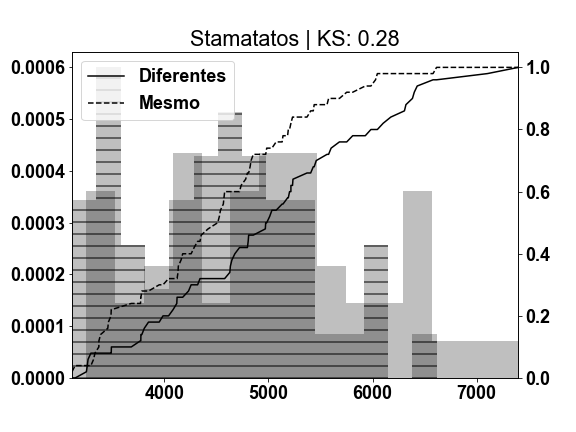
\includegraphics[width=.45\textwidth]{experimentoVerificacao/HDRIO_KS_spanish_Stamatatos.png} \vspace{0.3cm}
	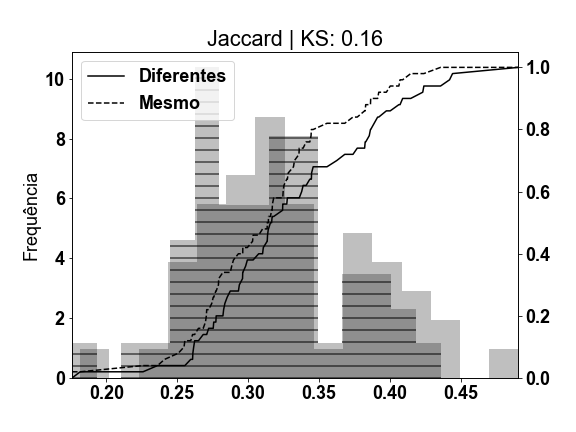
\includegraphics[width=.45\textwidth]{experimentoVerificacao/HDRIO_KS_spanish_Jaccard.png} \vspace{0.3cm}
	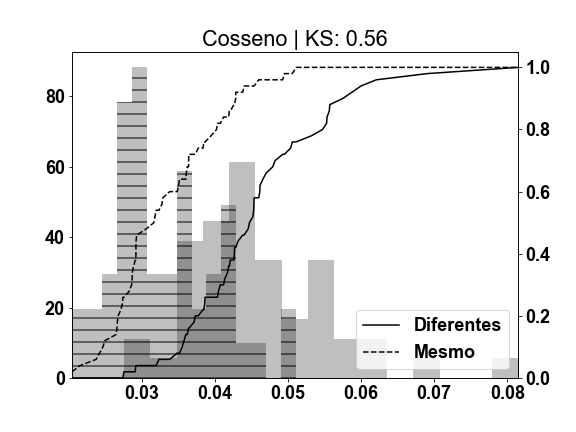
\includegraphics[width=.45\textwidth]{experimentoVerificacao/HDRIO_KS_spanish_Cosseno.png}
	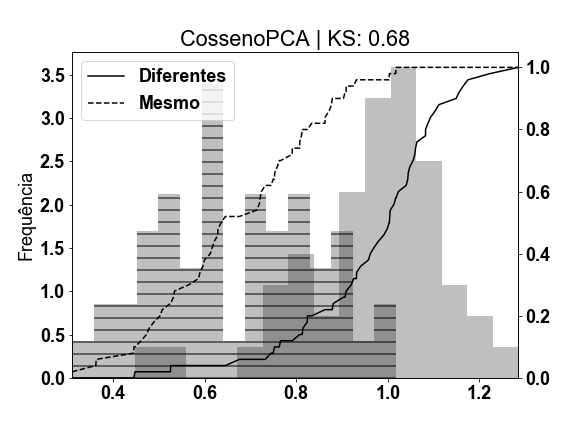
\includegraphics[width=.45\textwidth]{experimentoVerificacao/HDRIO_KS_spanish_CossenoPCA.png}
	\label{fig:exemplo}
\end{figure}
\end{column}
\begin{column}{0.37\textwidth}

\begin{itemize}
	\item Histograma para mesma autoria (tracejado).
	\item Histograma para autorias diferentes (liso).
	\item Distribuição acumuladas (linhas).
	\item Separação pela métrica Kolmogorov-Smirnov.
	\item Métricas AUC e acurácia.
\end{itemize}
\end{column}
\end{columns}


\end{frame}
\begin{frame}{Experimento 1: Verificação autoral}
\begin{block}{Modelo proposto 1 - MP1}
\begin{itemize}
\item As distâncias foram utilizadas como variáveis para o modelo.
\item Aplicado a normalização minmax.
\item Aplicado a regressão logística.
\end{itemize}
\end{block}
\begin{block}{Modelo proposto 2 - MP2}
\begin{itemize}
\item Os documentos conhecidos $C$ e de autoria desconhecidas $D$ foram unificados em um úncio BoW através da equação:
\begin{equation}
MP2\left ( C_{ij}, D_{ij} \right ) = \log\left ( 1 + \frac{\left ( C_{ij}-D_{ij} \right )^2}{C_{ij}+1} \right )
\label{eq:verificacao.mp2}
\end{equation}
\item Aplicado a normalização minmax.
\item Aplicado a regressão logística.
\end{itemize}		
\end{block}	
\end{frame}

\begin{frame}{Experimento 1: Verificação autoral}
\begin{table}[!htbp]
\centering
\caption{Verificação autoral - Resultados médios das métricas AUC e acurácia em 5-partições.}
\begin{tabular}{l|cc|cc}
\toprule
\multirow{2}{*}{\bf Modelo} & \multicolumn{2}{c|}{\bf PAN2014 (EE e EM)} & \multicolumn{2}{c}  {\bf PAN2014{-}SP} \\ \cline{2-5}
& {\bf ROC}  &        {\bf Acurácia}         & {\bf ROC}  &      {\bf Acurácia}       \\ \hline
Jaccard                     &    0,60    &             0,56              &    0,57    &           0,52            \\
Cossenos                    &    0,63    &             0,50              &    0,88    &           0,77            \\
Cossenos\_PCA               &    0,63    &             0,55              & {\bf 0,92} &        {\bf 0,83}         \\
Keselj                      &    0,61    &             0,54              &    0,71    &           0,60            \\
Stamatatos                  &    0,60    &             0,55              &    0,59    &           0,54            \\ \hline
MP1 – Mix                   & {\bf 0,75} &          {\bf 0,67}           &    0,72    &           0,62            \\
MP2 – BOW                   &    0,62    &             0,53              & {\bf 0,93} &        {\bf 0,85}         \\ \bottomrule
\end{tabular} 
\label{tab.results.verificacao}
\end{table}

{\selectFont
PAN2014 (EE e EM) córpus com textos em língua inglesa, PAN2014{-}SP textos em língua espanhola.
}
\end{frame}


%*******************************************************************
\begin{frame}{Experimento 2: Atribuição Autoral}
\begin{block}{Publicação 2}
CUSTÓDIO, J. E.; PARABONI, I. EACH-USP Ensemble Cross-domain Authorship
Attribution: Notebook for PAN at CLEF 2018. In: CAPPELLATO, L. et al. (Ed.).
Working Notes Papers of the CLEF 2018 Evaluation Labs. [S.l.]: CLEF and CEUR-WS.org,
2018. (CEUR Workshop Proceedings). ISSN 1613-0073.
\end{block}

\begin{block}{Atribuição por aprendizado de máquina supervisionado}
\begin{itemize}
\item Tem-se um conjunto de documentos para os quais se sabe quem são os autores e um documento do qual deseja-se atribuir.
\item O classificador extrai a ``assinatura do estilo''.
\item Aspectos inconscientes, como a sintaxe, são mais importantes que a semântica.
\item O trabalho apresentado foi parte da participação da tarefa de AA da competição PAN-CLEF2018.
\end{itemize}
\end{block}
\end{frame}

\begin{frame}{Experimento 2: Atribuição Autoral}
\begin{block}{Baseline {\it Bas.PAN}}
Os organizadores forneceram um sistema {\it baseline} pelos com as seguintes características:
\begin{itemize}
\item N-gramas de caracteres de tamanho fixo.
\item Normalização no documento por TF.
\item Sem normalização no córpus.
\item Frequência mínima de 4 ocorrências.
\item Classificador SVM encapsulado nas estratégias um-contra-um e um-contra-todos.
\item Foi otimizado por {\it grid search} com validação cruzada com 5 partições, e os melhores parâmetros foram:
\begin{itemize}\selectFont
\item n-gramas de tamanho 4.
\item Frequência mínima de 5 documentos.
\item SVM com estratégia um-contra-todos.
\end{itemize}
\end{itemize}
\end{block}
\end{frame}

\begin{frame}{Experimento 2: Atribuição Autoral}
Dado nossas premissas, o sistema final PAN2018 para AA consistiu de um comitê que concatenou as fontes de informações em uma saída única.

\begin{figure}[]\selectFont
\caption{\selectFont Método proposto final}
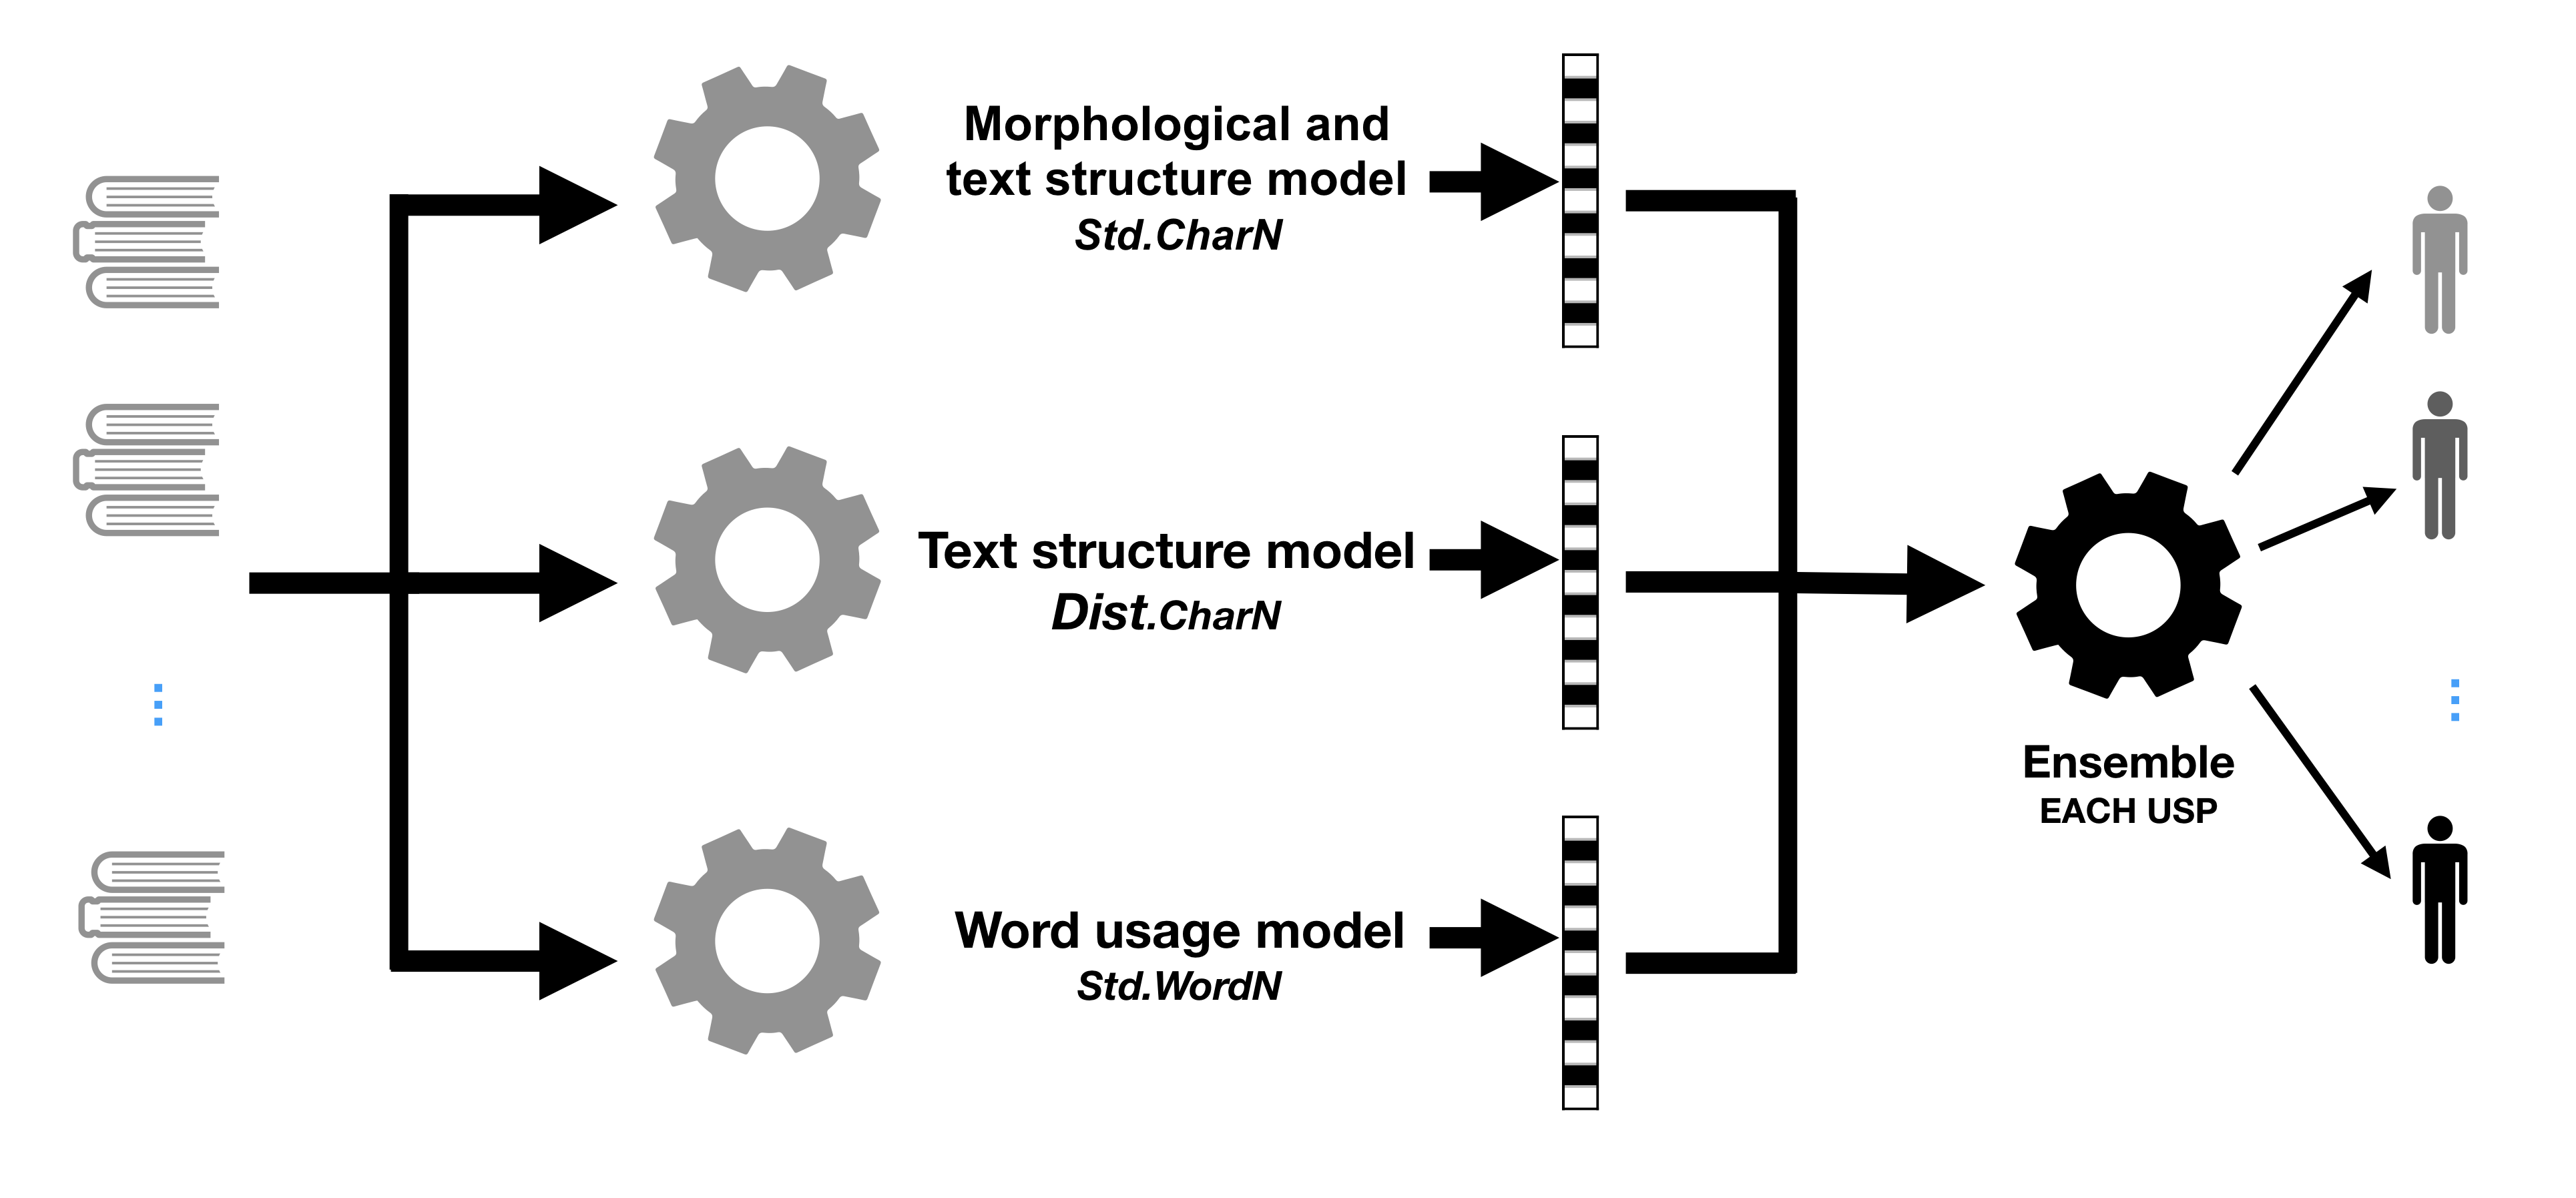
\includegraphics[width=.7\textwidth]{images/prop1_Diagramas.png}
\end{figure}

O sistema foi otimizado por {\it grid search} com validação cruzada de 5 partições.
\end{frame}

\begin{frame}{Experimento 2: Atribuição Autoral}
Premissa: O estilo de escrita de autor pode ser capturado através de diversas fontes de informação, como sintática, léxica e semântica.
\begin{block}{Método proposto {\it Std.word}}
Consistiu de um modelo BOW de n-gramas de palavras tradicional.
\end{block}
\begin{block}{Método proposto {\it Std.char}}
Consistiu de um modelo BOW de n-gramas de caracteres tradicional.
\end{block}
\begin{block}{Método proposto {\it Dist.char}}
Consistiu de um modelo BOW de n-gramas de caracteres onde são letras maiúscula e minúsculas sem acento são distorcidas, deixando a pontuação, espaços e letras com diacríticos.
\end{block}
\end{frame}

\begin{frame}{Experimento 2: Atribuição Autoral}
\selectFont
\setlength{\tabcolsep}{3pt}
\begin{table}[!htbp]
\centering
\caption{\selectFont Valores ótimos encontrados para PAN2018}
\begin{tabular}{m{2.2cm}m{4cm}m{4cm}}
\toprule
\textbf{Módulo} & \textbf{Parâmetros} & \textbf{Valores ótimos} \\ 
\midrule
\multirow{6}{2.2cm}{\bf Extração de características} & Faixa n-gram & 
\begin{tabular}[c]{@{}l@{ - }l@{}}
Std.charN &  Início=2 Fim=5\\
Dist.charN & Início=2 Fim=5\\
Std.WordN & Início=1 Fim=3\end{tabular}\\ 
& Freq. min. doc. & 0,05 \\ %\cline{2-3} 
& Freq. max. doc. & 1,0 \\ %\cline{2-3} 
& TF & Sublinear \\ %\cline{2-3} 
& IDF & Suavizado \\ %\cline{2-3} 
& Normalização no documento & L2 \\ 
\hline
{\bf Transformação} & PCA & 0,99 \\ 
\bottomrule
\end{tabular}
\label{tab.optimal}
\end{table}
\end{frame}

\begin{frame}{Experimento 2: Resultados obtidos em treinamento}
\setlength{\tabcolsep}{4pt}\selectFont
\begin{table}[!htbp]
\centering
\caption{\selectFont F1 para PAN-CLEF 2018 AA no córpus de desenvolvimento}
\begin{tabular}{ccc ccccc}
\bottomrule
{Problema} & {Língua} & {Autores} & {Bas.PAN} & {Std.charN} & {Dist.charN} & {Std.wordN} &   {Comitê}   \\ \midrule
01     &    EN    &    20     & 0,514     &    0,609    &    0,479     &    0,444    & {\bf 0,625}  \\
02     &    EN    &     5     & 0,626     &    0,535    &    0,333     &    0,577    & {\bf 0,673}  \\
03     &    FR    &    20     & 0,631     &    0,681    &    0,568     &    0,418    & {\bf 0,776}  \\
04     &    FR    &     5     & 0,747     &    0,719    &    0,586     &    0,572    & {\bf 0,820}  \\
05     &    IT    &    20     & 0,529     &    0,597    &    0,491     &    0,497    & {\bf 0,578}  \\
06     &    IT    &     5     & 0,614     &    0,623    &    0,595     &    0,520    & {\bf 0,663}  \\
07     &    PL    &    20     & 0,455     &    0,470    &    0,496     &    0,475    &   { 0,554}   \\
08     &    PL    &     5     & 0,703     & {\bf 0,948} &    0,570     &    {\bf 0,922}    &    0,922     \\
09     &    ES    &    20     & 0,709     & {\bf 0,774} &    0,589     &    0,616    &    0,701     \\
10     &    ES    &     5     & 0,593     &    0,778    &   {\bf 0,802} &    0,588    & {\bf 0,830}  \\ \bottomrule
Média    &          &           & 0,612     &    0,673    &    0,551     &    0,563    & {\bf 0,714 } \\ \bottomrule
\end{tabular}
\label{tab.results}
\end{table}
\end{frame}


\begin{frame}{Experimento 2: Resultados obtidos em produção}
\selectFont

Resultado geral apresentados pelos organizadores do PAN2018 \cite{aa-overview-2018}.

\setlength{\tabcolsep}{3pt}\selectFont
\begin{table}[]
\centering
\caption{\selectFont PAN-CLEF 2018 - 3 melhores equipes - por língua}
\begin{tabular}{m{5cm}cccccc}
	\toprule
	{\bf Equipe}                      & {\bf F1 Geral} &  {\bf EN}   &  {\bf FR}   &  {\bf IT}   & {\bf PL} &  {\bf ES}   \\ \midrule
	\citeonline{custodioParaboni2018} &  {\bf 0,685}   &    0,744    & {\bf 0,668} &    0,676    &  0,482   & {\bf 0,856} \\
	\citeonline{Murauer2018}          &     0,643      & {\bf 0,762} &    0,607    &    0,663    &  0,450   &    0,734    \\
	\citeonline{Halvani2018}          &     0,629      &    0,679    &    0,536    & {\bf 0,752} &  0,426   &    0,751    \\
	PAN18-BASELINE                    &     0,584      &    0,697    &    0,585    &    0,605    &  0,419   &    0,615    \\ \bottomrule
\end{tabular}

\caption{\selectFont PAN-CLEF 2018 - 3 melhores equipes - por língua}
\begin{tabular}{m{5cm}cccc}
	\toprule
	{}                                &     \multicolumn{4}{c}{\bf Quantidade de autores}     \\ \cline{2-5}
	{\bf Equipe}                      &  {\bf 20 }  &  {\bf 15 }  &  {\bf 10 }  &  {\bf 5 }   \\ \midrule
	\citeonline{custodioParaboni2018} & {\bf 0,648} & {\bf 0,676} & {\bf 0,739} & {\bf 0,677} \\
	\citeonline{Murauer2018}          &    0,609    &    0,642    &    0,680    &    0,642    \\
	\citeonline{Halvani2018}          &    0,609    &    0,605    &    0,665    &    0,636    \\
	PAN18-BASELINE                    &    0,546    &    0,532    &    0,595    &    0,663    \\ \bottomrule
\end{tabular}
\label{tab.experimento1.resultados.por.autores}
\end{table}
\end{frame}
